\documentclass[11pt]{article}
\usepackage{graphicx}
\usepackage[utf8]{inputenc}
\usepackage{geometry}
\usepackage{titlesec}
\usepackage{enumitem}
\usepackage{hyperref} 
\usepackage{amsmath}
\usepackage{ gensymb }
\usepackage{ amssymb }
% \usepackage{parskip}
\usepackage{float}
\usepackage{amsthm}
\usepackage{tikz}
\usepackage{float}
\usepackage[colorinlistoftodos]{todonotes}
\usepackage{algorithm}
\usepackage{tikz}
\usetikzlibrary{matrix, decorations.pathreplacing}
\usepackage{algpseudocode}

\setlength{\parindent}{0pt}

\theoremstyle{definition}
\newtheorem{definition}{Definition}[section]
\newtheorem{remark}{Remark}[section]


\newcommand{\R}{\mathbb{R}}
\newcommand{\N}{\mathbb{N}}
\newcommand{\C}{\mathbb{C}}
\newcommand{\Q}{\mathbb{Q}}
\newcommand{\Z}{\mathbff{Z}}
\newcommand{\st}{\text{s.t}}
\newcommand{\bigO}[1]{\mathcal{O}\left(#1\right)}

\title{STAT 24310 Notes}
\author{Anthony Yoon}
\begin{document}
\maketitle
\begin{abstract}
  Notes for STAT 24310 taught by Professor Yuehaw Khoo. Prior Linear Algebra and some basic multivariate calculus knowledge will be assumed.  MATLAB notation for matrices will be extensively used. 
\end{abstract}
\tableofcontents
\newpage
\section{Lecture 1: Introduction}
This class is heavily based on \href{https://www.stat.uchicago.edu/~lekheng/courses/309/books/Trefethen-Bau.pdf}{Trefethen and Bau's Textbook}. Take a look at it if you have the time. \\
When we run an algorithm, we often are interested in how long it takes to run the algorithm. For example, if we have a matrix $A \in \R^{n \times n}$ an $x, b \in \R^n$, and we are interested in solving 
\[
Ax = b
\]
and $n$ is very large, say $ n = 100,000$, a concern is that the algorithm takes forever to run. In this case, we may be worried about the worst case time complexity, denoted as \emph{big O notation}. In this case, solving $x = A^{-1} b$ is $\mathcal{O}(n^3)$. But what is this notation? 
\begin{definition}
  If there exists a $C \in \R$ such that for $f g$, where $g \geq 0$, where for all sufficiently $t$ large enough, such that $|f(t)| \leq C \cdot g(t)$, then $f(t) \mathcal{O}(g(t))$ 
\end{definition}
or equivantly:
\begin{definition}
  If there exists a constant \( C \in \mathbb{R} \) and a real number \( t_0 \) such that for all \( t \geq t_0 \), \( |f(t)| \leq C \cdot g(t) \), where \( g(t) \geq 0 \), then we write \( f(t) = \mathcal{O}(g(t)) \) as \( t \to \infty \).
\end{definition}
Both are equivalent. For example, consider a problem that is $\mathcal{O}(n^3)$. If we were to increase the dimension of the problem, say a 100 times, then the algorithm would take 10000000 times longer to run. However, how do we visualize this? We do so by plotting the log-log plot, where we can note that:
\begin{align*}
  t &= \mathcal{O}(n^3)\\
  \log t &= 3 \log n + C
\end{align*}
where $C$ is some constant. 
\begin{center}
  \begin{tikzpicture}[scale=1.5]
    % Draw axes
    \draw[->] (0,0) -- (3,0) node[right] {$\log n$};
    \draw[->] (0,0) -- (0,3) node[above] {$\log t$};
    
    % Draw the line y = x
    \draw[thick, domain=0:3] plot (\x,\x);
    
    % Add ticks if you want
    \foreach \x in {1,2}
      \draw (\x,0.05) -- (\x,-0.05) node[below] {\small $\x$};
    \foreach \y in {1,2}
      \draw (0.05,\y) -- (-0.05,\y) node[left] {\small $\y$};
  \end{tikzpicture}

\end{center}
where we can see that the slope gives the exponent in time complexity. 
\subsection{Accuracy} 
When we are dealing with algorithms, we can also be concerned with how accurate it is. For example, consider $f: X \to Y$, where we are interested $f(x)$ for $x \in X$. However, pratically, we cannot calculate the exact values, take $\sqrt{x}$ for example, so a computer must make an approximation, usually denoted as $\tilde{f}(x)$. We can consider the relative accuracy, defined as follows:
\begin{definition}
  Given an approximation of a function $\tilde{f}(x)$, we define relative accuracy as:
  \[
  \frac{\|\tilde{f}(x) - f(x)\|}{\|f(x)\|}
  \]
  where $\| \cdot \|$ is the norm of choosing. 
\end{definition}
A natural extension of accuracy are the follwing topics: \textbf{Stability and Conditional Number}. Intuively, stability is usually related to the algorithm $(\tilde{f}(x))$ used to solve the problem and the condition number is related to the actual setup of the problem $(f(x))$. We can consider the following defintions:
\begin{definition}
  Backwards Stability: if $x \in X$. $\tilde{f}(x) = f(\tilde{x})$ for some $\frac{\| \tilde{x} - x \|}{\|x\|} = \mathcal{O}(\epsilon)$
\end{definition}
Intuively, this above definition says that the problem will give the good enough answer to a slight deviation in the input. This definition is usually easier to prove. 
\begin{definition}
  Absoulte Conditional Number: for $(f, x)$l we can consider the Absolute condition number as follows:
  \[
  \hat{K}(f, x) = \lim_{\delta \to 0} \sup_{\|\delta x \| \leq \delta} \frac{\|f(x+\delta x) -f(x)\|}{\|\delta x\|} 
  \]
\end{definition}
\begin{definition}
  Relative Conditional Number: for $(f,x)$, we define the relative condition number as:
  \[
  \lim_{\delta \to 0} \sup_{\frac{\| \delta x \|}{\|x\|} \leq \delta} \frac{\frac{\|f(x + \delta) - f(x)\|}{\|f(x)\|}}{\frac{\| \delta x \|}{\|x\|}} = \frac{\|f(x+ \delta x) - f(x)\| \|x\|}{\| f(x) \| \|\delta x \|}
  \]
\end{definition}
We can consider the diagram as follows:
\begin{center}
  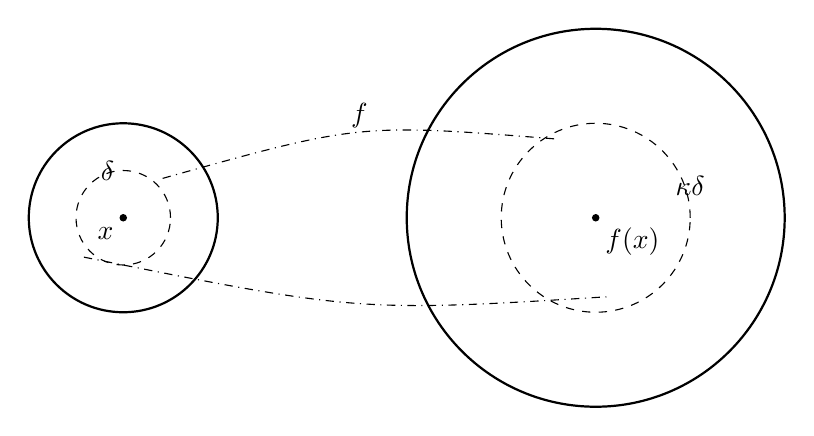
\begin{tikzpicture}[scale=2]

    % Left side: domain space
    \coordinate (x) at (0,0);
    \draw[fill=black] (x) circle (0.02) node[below left] {$x$};
    \draw[dashed] (x) circle (0.3); % inner delta ball
    \node at (-0.1,0.3) {$\delta$};
    \draw[thick] (x) circle (0.6); % outer bound
  
    % Right side: codomain space
    \coordinate (fx) at (3,0);
    \draw[fill=black] (fx) circle (0.02) node[below right] {$f(x)$};
    \draw[dashed] (fx) circle (0.6); % inner k delta ball
    \node at (3.6,0.2) {$\kappa \delta$};
    \draw[thick] (fx) circle (1.2); % outer bound
  
    % Arrows showing mapping
    \draw[dash dot] (0.25,0.25) .. controls (1.5,0.6) .. (2.75,0.5);
    \draw[dash dot] (-0.25,-0.25) .. controls (1.5,-0.6) .. (3.1,-0.5);
  
    % Label for mapping
    \node at (1.5, 0.65) {$f$};
  
  \end{tikzpicture}
\end{center}
We can see that the condition number measures how senstive the actual problem is to a change in $x$, as seen above. The larger the problem is, the more sensitive the problem is. Think of the diameter of the circles as how values go between each set. If the condition number is large, then the diameter is larger and thus, there is chance that the small pertrepuabation lands in a different area than original output. 
\begin{remark}
  Note if $f$ is a function from $\R^n - \R^m$, we can define the following:
  \[
  K_{abs} = J_f \quad K_{rel} = J_f \cdot \frac{\|x\|}{\|f(x)\|}
  \]
\end{remark}


We can observe the following. If $\tilde{f}$ is backwards stable with accuracy $\epsilon$, and if $f$ has a relative condition number $k$. then $\tilde{f}$ is accurate with the follwoing relation:
\[
\frac{\| \tilde{f}(x) - f(x) \|}{\|f(x)\|} = \mathcal{O}(k \epsilon)
\]
\begin{proof}

  If \( \tilde{f} \) is backward stable, then there exists a point \( y \in (x - \delta, x + \delta) \), with \( \|\delta\| = \mathcal{O}(\epsilon \|x\|) \), such that:
  \[
  \tilde{f}(x) = f(y)
  \]
  This means the computed value \( \tilde{f}(x) \) is the exact value of \( f \) evaluated at a slightly perturbed input \( y \).
  
  Now, using the definition of the relative condition number \( \kappa \) of \( f \), we know that for small perturbations:
  \[
  \frac{\|f(y) - f(x)\|}{\|f(x)\|} \leq \kappa \cdot \frac{\|y - x\|}{\|x\|} + \mathcal{O}\left(\left(\frac{\|y - x\|}{\|x\|}\right)^2\right)
  \]
  Since \( \|y - x\| / \|x\| = \mathcal{O}(\epsilon) \), it follows that:
  \[
  \frac{\|\tilde{f}(x) - f(x)\|}{\|f(x)\|} 
  = \frac{\|f(y) - f(x)\|}{\|f(x)\|} 
  = \mathcal{O}(\kappa \epsilon)
  \]
\end{proof}
\section{Lecture 2: Norms}
We begin with following definition of a norm in a general vector space. 
\begin{definition}
  Let $X$ denote a vector space. A norm $\| \cdot \| : X \to R$ sastisfies
  \begin{itemize}
    \item Positivity: $\| x\| \geq 0$, $\| x \| = 0$ iff $x = 0$
    \item Homogenuity: $\| \alpha x \| = |alpha| \| x \|$ 
    \item Triangle inquality: $\| x + y \| \leq \| x \| + \| y \|$
  \end{itemize}
\end{definition}
We can also define the $l_p$ norm
\begin{definition}
  The $l_p$ is defined as:
  \begin{itemize}
    \item $\| x\|_p = \left( \sum_{i = 1}^{n} |x_i|^p \right)^\frac{1}{p}$, where $0 < p < \infty$
    \item $\|x \|_0$ refers to number of non-zero elements of $X$. 
    \item $\| x \|_\infty = \max_j \{ |x_j| \}$
  \end{itemize}
\end{definition}
We also have the following definitions: 
\begin{definition}
  Inner product on $\C^n$: $\langle x, y \rangle = \sum_{i = 1}^{m} \overline{x}_i y_i$
\end{definition}
\begin{definition}
  Cauchy Schwartz inequality: $| \langle x, y \rangle | \leq \|x \| \|y \|$
\end{definition}

\begin{definition}
  Holder's inequality: $| \langle x, y \rangle \leq \|x\|_p \|y\|_q$ is $\frac{1}{p} + \frac{1}{q} = 1$
\end{definition}
We can also define the equivalence of norms:
\begin{definition}
  $\| \cdot \|_a, \| \cdot \|_b$ are equivalent if for $c_2 \geq c_1 \geq 0$:
  \[
  C_1 \|x \|_b \leq \|x \|_a \leq C_2 \|x\|_b
  \]
\end{definition}
We can prove that all norms are equivalent. This will be left as an exercise to the reader. 
\subsection{Matrix Norms}
We can also introduce the notion of norms on matrices. 
\begin{definition}
  Frobenious norm: $\|A \|_F = \left( \sum_{i = 1, j = 1}^{m, n} |A_{ij}|^2 \right)^\frac{1}{2}$
\end{definition}
\begin{definition}
  Induced norm: Given $A \in \C^{m \times n }, x \in \C^n$. We define the induced norm as follows:
  \[
  \|A \|_{a \to b} = \sup_{x \neq 0} \frac{\|Ax\|_a}{\|x\|_b} = \sup_{\|x\|_b = 1} \|Ax \|_a
  \]
\end{definition}
\begin{remark}
  By definition, we can see that: 
  \[
  \|Ax \|_a \leq \|A\|_{a \to b} \|x\|_b \quad \|A\|_a = \|A\|_{a \to a}
  \]
\end{remark}
We also have the follwing properties:
\begin{definition}
  We can also denote the following p norms. 
  \begin{itemize}
    \item $\|A\|_1 = \max_{1 \leq j \leq n} \| A(:,j)\|_1$, which is just the maximum column sum.
    \item $\|A\|_\infty = \max_{1 \leq i \leq m} \|A(i, :)\|_1$  Which is the max of the row sum. 
  \end{itemize}
\end{definition}
We also have the Cauchy Schwartz inequality for the matrix norm:
\begin{definition}
  $\|AB\|_2 \leq \|A\|_2 \|B\|_2$ and $\|AB\|_f \leq \|A\|_F\|B\|_f$ and $\|AB\|_f \leq \|A\|_2 \|B\|_F$
\end{definition}
We can prove the fact $\|AB\|_2 \leq \|A\|_2 \|B\|_2$, which is as follows:
\begin{proof}
  $\|AB\|_2 \leq \|A\|_2 \|B\|_2$. To show this note, 
  \begin{align*}
    \sup_{\|x \| = 1} \|ABx\|_2 & \leq \|Ay\|_2 \leq \| A\|_2 \|y\|_2 \leq \|A\|_2 
  \end{align*}
\end{proof}
\section{3: linear Transform}
In numerical linear algebra, most problems and algorithms consist of linear maps. 
\begin{definition}
  Linear Transform is a function from $T: X \to Y$ where
  \begin{itemize}
    \item $T(\alpha x + \beta y) = \alpha T(x) + \beta T(y)$ 
    \item $T(v) = Av$ where $A \in \C^{m \times n}, v \in \C^n$
  \end{itemize}
\end{definition}
For example consider the following example. \\
\textbf{Example}\\
Let $P_k(x) = x^k$, where it is monomial, where $k \in \N \cup \{ 0\}$, where $X = span \{ P_0, P_1, P_2\}$ and $Y = span \{P_0, P_1, P_2, P_3$. Note that if $q \in X$. this means that $q$ is equivalent to a linear combination of the polynomials, where we can see that $Tq = (q + 1)q$ It is trivial to show that $T$ is a linear transform. Thus, we aim to find the matrix for this. Consider the following
\[
Tp_1 = p_2 + p_1 \quad Tp_2 = p_3 + p_2
\] 
where we can construct the matrix as follows\footnote{Professor Khoo did some weird proof about the change of basis here, and frankly I don't think its worth putting here as an FYI}
\[
A = \begin{bmatrix}
  1 & 0 & 0\\
  1 & 1 & 0 \\
  0 & 1 & 1\\
  0 & 0 & 1
\end{bmatrix}
\]
where columns vector is $\{p_0, p_1, p_2, p_3\}$ and row vectors are $\{p_0, p_1, p_2\}$. 
\subsection{Inner Products}
We can introduce the inner product as follos. 
\begin{definition}
  Given a inner product $\langle \cdot , \cdot \rangle $ where $v \in \C^n$, we can see that 
  \begin{itemize}
    \item It sastifies bilinearity 
    \item $\langle v, w \rangle = \langle w , v \rangle$
    \item $\langle v, v \rangle \geq 0$ if and only if $v = 0$
  \end{itemize}
  Note that $\langle v, v \rangle = \| v \|^2$ . We can also define $\langle v, v \rangle_M = v^T M V$ where $M$ is a positive definite matrix.
\end{definition}
\begin{definition}
  A matrix is positive definite if and only if all the eigenvalues are positive. 
\end{definition}
\begin{definition}
  A matrix is negative definite if and only if all the eigenvalues are negative. 
\end{definition}
\begin{definition}
  Hermitian matrix is the complex analgue to the transpose of a matrix. Symmmetric matrix is $A^T = A$ and Hermitian matrix is $A = A^*$ \footnote{The ${}^*$ superscript denotes the complex conjugate, where every entry of the matrix is conjugated.}
\end{definition}
\subsection{Different kinds of multiplication}
Refer to my \href{https://github.com/anthonykyoon/notes-latex/blob/main/notes/STAT24300.pdf}{STAT 24300} notes. Covers all the definition in Lectures 1 and 5. The only extension we have to be concerned about is the complexity of each operation. We can characterize it as follows:
\begin{itemize}
  \item Inner product $\bigO{n}$, as we are multiplying ad summing $n$ times
  \item Matrix vector product is $\bigO{mn}$ as we are doing the dot product over $m$ rows. 
  \item Matrix Matrix product is $\bigO{mnp}$, where $A \in \C^{m \times n}, B \in \C^{n \times p}$, as we are doing matrix vector product $p$ times. 
\end{itemize}
\section{4: Conditioning of the Linear Transform}
Let us consider $T(x) = Ax$. To analyze behavior of the matrix, we decompose is $A = F_1 F_2 \dots F_n$. We have the following key decompositions. 
\begin{itemize}
  \item For a square matrix, we have Eigenvalue Decomposition (EVD), where if we have a diagnolzaible matrix A where\footnote{Diag is shorthand for a diagnol matrix} \[
  A = V \Lambda V^{-1} \quad \Lambda = diag(\lambda_1, \lambda_2, \dots, \lambda_n)
  \]
  where $V$ have columns are linearly independent vectors. Let $v_i$ be a column of the eigenbasis, then we see that $Av_i = \lambda_i v_i$ as 
  \[
  \det(A - \lambda I) = 0 \implies \quad \exists \quad v \st \quad (A - \lambda I)v = 0 \iff Av = \lambda v
  \]
  \item SVD, where we have $A \in \C^{m \times n}$ where $A = U \Sigma V^*$, where $U \in \C^{m \times m}$ and $\Sigma \in \C^{m \times n}$ and $V \in \C^{n \times n}$ and where $\Sigma = diag(\sigma_1, \sigma_2, \dots, \sigma_n)$. 
\end{itemize}
The SVD is something that we discuss heavily in this class. For the time being, assume that $U$ and $V$ is unitary, which means that $U^T U = V^T V = I_n$. This will be covered later. For both cases, the number of eigenvaues or singular values equals the rank of the matrix. 
\subsection{Spectral Radius}
Given a matrix $A \in \C^{n \times n}$, we can define the spectral norm
\begin{definition}
  We define the spectral norm as 
  \[
  \rho (A) := \max_{j \in \{1, 2, \dots, m\}} \left| \lambda_j(A)\right|
  \]
\end{definition}
\begin{remark}
  Note that $\|A\|_p \geq \rho(A)$. As let $v$ be an eigenvector of A,
  \begin{align*}
    \|Av\|_p = \|\lambda v \|_p &\leq \|A\|_p \|v\|_p \\
    |\lambda| &\leq \|A\|_p
  \end{align*}
\end{remark}
We can prove that $\|A\|_2^2 = \sigma_1$.
\begin{proof}
  Let \( A \in \mathbb{C}^{m \times n} \), and let the singular value decomposition (SVD) of \( A \) be:

\[
A = U \Sigma V^*
\]

where:
\begin{itemize}
    \item \( U \in \mathbb{C}^{m \times m} \), \( U^* U = I_m \) (unitary),
    \item \( V \in \mathbb{C}^{n \times n} \), \( V^* V = I_n \) (unitary),
    \item \( \Sigma \in \mathbb{R}^{m \times n} \) is diagonal with nonnegative entries \( \sigma_1 \geq \sigma_2 \geq \cdots \geq \sigma_r > 0 \), the singular values of \( A \).
\end{itemize}

Recall that the operator 2-norm (spectral norm) of \( A \) is defined by:

\[
\|A\|_2 := \sup_{\|x\|_2 = 1} \|Ax\|_2
\]

Using the SVD \( A = U \Sigma V^* \), and noting that \( U \) and \( V \) are unitary (thus preserve the 2-norm), we compute:

\[
\|A\|_2 = \sup_{\|x\|_2 = 1} \|A x\|_2 
= \sup_{\|x\|_2 = 1} \|U \Sigma V^* x\|_2
= \sup_{\|x\|_2 = 1} \|\Sigma V^* x\|_2
\]

Let \( y = V^* x \). Since \( V \) is unitary, \( \|y\|_2 = \|x\|_2 = 1 \). So:

\[
\|A\|_2 = \sup_{\|y\|_2 = 1} \|\Sigma y\|_2
\]

Now, \( \Sigma \) is a diagonal matrix with singular values \( \sigma_1, \dots, \sigma_r \), so for any unit vector \( y = (y_1, \dots, y_n) \), we have:

\[
\|\Sigma y\|_2^2 = \sum_{i=1}^{r} \sigma_i^2 |y_i|^2 \leq \sigma_1^2 \sum_{i=1}^{r} |y_i|^2 \leq \sigma_1^2
\]

The supremum is achieved when \( y = e_1 \), so:

\[
\|A\|_2^2 = \sup_{\|y\|_2 = 1} \|\Sigma y\|_2^2 = \sigma_1^2
\]
\end{proof}
Using a very similar logic, we can see that $\|A^{-1}\|_2 = \frac{1}{\sigma_n}$
\section{Lecture 5: Unitary Matrix}
We begin with the proof of the unitary matrix. 
\begin{proof}
  Consider the definition of the relative condition number, where we see that 
  \[
  K = \lim_{\delta \to 0} \sup_{\|\delta x\| \leq \delta} \frac{\|x\|}{\|Ax\|} \frac{\|A \delta x\|}{\| \delta x\|}
  \]
  and we see that the above is equivalent to:
  \[
  k(A) = \|A^{-1}\| \|A\|
  \]
  Note that if $\| \cdot \| = \| \cdot \|_2$, then we see that:
  \[
  k_{rel} = \frac{\sigma_1}{\sigma_n}
  \]
\end{proof}
now we can proceed to the properties of the Unitary matrix. First, we can introduce the properties of an orthogonal matrix:
\begin{definition}
  Let \( Q \in \mathbb{R}^{m \times n} \) with \( m > n \), where $q_i$ denotes the columns of $Q$. we see that $\forall q_i$, $\|q_i\| = 1$, $\langle q_1 , q_j \rangle = \delta_{ij}$. A such matrix is called orthonormal. 
\end{definition}
\begin{definition}
 A matrix that is orthonormal and square is unitary. 
\end{definition}
We can see the following properties of orthonormal and orthogonal matrices, where $Q^* Q = I_n$, $K(Q) = 1$ and $\|Qx\|_2 = \|x\|_2$
\subsection{Basis interpretation of Q being orthogonal}
Let $x = Qz$, where $z \in \C^n$. We assume that $Q$ is an unitary matrix and $x \in Range(Q)$. Thus, we see that by the definition of matrix vector multiplication, we see that:
\[
x = \sum_{i = 1}^{n} z_i Q_i
\]
However, note that:
\[
\langle Q_i, x \rangle = \langle Q_i , \sum_{i = 1}^{n} z_i Q_i \rangle = \sum_{i = 1}^{n} z_i \langle Q_i, Q_j \rangle 
\]
Thus, using this idea, we can see that 
\begin{align*}
  x &= \sum_{i = 1}^{n} z_i Q_i\\
  &= \sum_{i = 1}^{n} Q_i \langle Q_i , x \rangle \\
  &= \sum_{i = 1}^{n} Q_i Q_i^* x
\end{align*}
thus, we can see that $Q Q^*$ acts like an indentity matrix. 
\begin{definition}
  We can see that if we let $Q$ to be orthonormal, we find that $QQ^*$ is the orthogonal projector to the subspace $span(Q_1, Q_2, \dots, Q_n) = range (Q)$ if $Q \not \in range(Q)$. 
\end{definition}
\begin{remark}
  We can see that $(I - QQ^*)v$ represents the perpendicular aspect of the vector, or rather the part that is not projected into the subspace.
\end{remark}
\section{Lecture 6: QR decomposition}
Refer to \href{https://en.wikipedia.org/wiki/Gram%E2%80%93Schmidt_process#The_Gram%E2%80%93Schmidt_process}{this article}, does a very good of explaning it. The intution is we keep removing all perpednicualr parts of each vector in the basis to ensure we have an orthonormla basis. We have the following algorthim to solve it. 

\begin{algorithm}[H]
  \caption{Gram-Schmidt Orthogonalization (Matrix Form)}
  \begin{algorithmic}[1]
  \Require Linearly independent vectors $\{a_1, a_2, \dots, a_n\} \subseteq \mathbb{C}^m$
  \Ensure Orthonormal matrix $Q = [q_1 \ q_2 \ \dots \ q_n] \in \mathbb{C}^{m \times n}$ such that $\text{span}(q_1, \dots, q_k) = \text{span}(a_1, \dots, a_k)$ for all $k$
  
  \State $q_1 \gets \dfrac{a_1}{\|a_1\|}$
  \For{$j = 2$ to $n$}
      \State Let $Q_{1:j-1} \gets [q_1 \ q_2 \ \dots \ q_{j-1}]$
      \State $v_j \gets \left(I - Q_{1:j-1} Q_{1:j-1}^*\right)a_j$
      \State $q_j \gets \dfrac{v_j}{\|v_j\|}$
  \EndFor
  \State \Return $Q = [q_1 \ q_2 \ \dots \ q_n]$
  \end{algorithmic}
\end{algorithm}
we can also find an upper triangular matrix of $A$, whose columns are $\{a_1, a_2, \dots a_n \}$, where we can consider the following algorithm\footnote{Not explicity explained by Professor Khoo, but nice to know}
\begin{algorithm}[H]
  \caption{QR Decomposition via Gram-Schmidt (Matrix Form)}
  \begin{algorithmic}[1]
  \Require Linearly independent vectors $\{a_1, a_2, \dots, a_n\} \subseteq \mathbb{C}^m$
  \Ensure $Q \in \mathbb{C}^{m \times n}$ with orthonormal columns, and upper triangular $R \in \mathbb{C}^{n \times n}$ such that $A = QR$
  
  \State Initialize $Q \gets 0_{m \times n}$, $R \gets 0_{n \times n}$
  \For{$j = 1$ to $n$}
      \State $v_j \gets a_j$
      \For{$i = 1$ to $j-1$}
          \State $R_{i,j} \gets \langle q_i, a_j \rangle$
          \State $v_j \gets v_j - R_{i,j} q_i$
      \EndFor
      \State $R_{j,j} \gets \|v_j\|$
      \State $q_j \gets \dfrac{v_j}{R_{j,j}}$
      \State Set column $j$ of $Q$ to $q_j$
  \EndFor
  \State \Return $(Q, R)$ such that $A = QR$
  \end{algorithmic}
\end{algorithm}
The complexity of calculating the norm is $\bigO{m}$. Note the matrix multiplciation of $Q_{1 : j-1}Q^*_{1:j-1}$ is $\bigO{m(j-1)}$. Thus, performing we can see that:
\[
\bigO{m} + \bigO{m(j-1)} + \bigO{m(j-1)} = \bigO{m + 2m(j-1)} = \bigO{m(j-1)} = \bigO{mn}
\]
note we do the operation $n$ times via the for loop, and we see that the final compleixty is $\bigO{mn^2}$. However, note the division sign. This means that algorithm is unstable as values could exponentially increase geivn a small enough norm magnitude. From here, we can introduce a more stable procedure, the Householder Reflection. 
\subsection{HouseHolder Relfection}
Refer to the visualzaition for intuition of the Householder transformation. 
\begin{figure}[H]
  \centering
  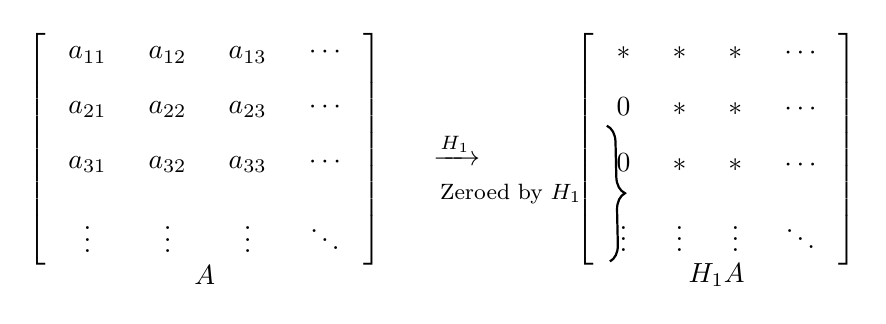
\begin{tikzpicture}
    % Original matrix A
    \matrix[matrix of math nodes, left delimiter={[}, right delimiter={]}, row sep=0.25cm, column sep=0.3cm] (A) at (0,0)
    {
      a_{11} & a_{12} & a_{13} & \cdots \\
      a_{21} & a_{22} & a_{23} & \cdots \\
      a_{31} & a_{32} & a_{33} & \cdots \\
      \vdots & \vdots & \vdots & \ddots \\
    };
  
    % Arrow indicating transformation
    \node at (3.2,0) {$\xrightarrow{H_1}$};
  
    % Transformed matrix HA
    \matrix[matrix of math nodes, left delimiter={[}, right delimiter={]}, row sep=0.25cm, column sep=0.3cm] (HA) at (6.5,0)
    {
      * & * & * & \cdots \\
      0 & * & * & \cdots \\
      0 & * & * & \cdots \\
      \vdots & \vdots & \vdots & \ddots \\
    };
  
    % Label A
    \node at (0,-1.6) {$A$};
    \node at (6.5,-1.6) {$H_1 A$};
  
    % Bracket and label for "Householder zeroed part"
    \draw[decorate,decoration={brace,amplitude=6pt}, thick] (HA-2-1.south west) -- (HA-4-1.south west)
      node[midway,left=6pt] {\footnotesize Zeroed by $H_1$};
  \end{tikzpicture}
\end{figure}
With the householder reflection decomposition, we aim to reduce problem of the QR decomposition to 
\[
A^{(1)} = Q^{(1)} A^{(0)} \quad A^{(2)} = Q^{(2)}A^{(1)}
\]
\[
Q^{(n)} Q^{(n-1)} \dots Q^{(1)} A = R
\]
where if $Q^{(i)}$ is an unitary matrix, that we are left with a QR factorization. 


We want our string of unitary matrices to be in the following form:
\[
Q^{(1)} = \begin{bmatrix}
  I_{j-1} & 0 \\ 0 & F^{(1)}
\end{bmatrix}
\]
where $F$ is $(m - j + 1) \times (m - j + 1)$. We want this $F$ to act on the lower half of $A$ to ensure that we elimnate the entries below to ensure that we have the RREF like structure of the above diagram. Or more specfically, 
\[
A^{(j-1)} = \begin{bmatrix}
  U^{(j-1)} \\ L^{(j-1)}
\end{bmatrix}
\]
where $U^{(j-1)}$ is $(j-1) \times (j-1)$ and $L^{(j-1)}$ is $(m - j + 1) \times (m - j + 1)$. Thus, we can see that:
\[
A^{(j-1)} = Q^{(j)} A^{(j-1)} = \begin{bmatrix}
  U^{(j-1)} \\ F^{(j)} L^{(j-1)}
\end{bmatrix} 
\]
We also want to make $F$ an orthonomral matrix to enforce that the bigger $Q$. However, to reinforce the RREF like nature, we have the following subproblem. 
\begin{center}
  We want to solve the problem of $Fx = z \|x\| e_1$
\end{center}
where $|z| = 1$.  Let $v = \|x\|e - x$, which we call the householder vector. The geonetric intuition of this is that $v$ points in the direction of $\|x\|e$ to from x, and we can reflect the point accross the line to get the vector mapped onto $\|x\|e$, which is equivalent to zeroing out entries. 
\begin{figure}[H]
    \centering
    \includegraphics[width=0.75\linewidth]{MOVETHIS.jpeg}
    \caption{Intution of the householder reflection}
    \label{fig:enter-label}
\end{figure}
However, we are interested in the quantity $v = \|x\|e - x$. Thus, we find the reflection matrix as follows: 
\[
I - \frac{2v v^*}{\|v\|^2} 
\]
where the multiplication of two is derived from the fact that we are interested in a vector pointing in the opposite direction original vector. Now, a natural question that may arise from this is \emph{what is the optimal choice of z?}. To ensure numeric stabilitty, we choose $z \in \{-1, 1\}$ such that $z$ has the opposite sign of $x$. The pseudocode for this decomposition is as follows:
\begin{algorithm}[H]
  \caption{Householder Relfection QR decomposition}
  \begin{algorithmic}[1]
    \Require $A \in \C^{m \times n}$
    \Ensure $Q_1 Q_2 \dots Q_n A = R$
    \State Let $A^{0} = A$
    \State Let $Q_0 = I_m$
    \State Intialize 
    \For{$j$ in $1:min(m,n)$}
      \State $x = A^{j-1}_{(j:m, j)}$
      \State Let z be opposite sign of x 
      \State Let $\tilde{v}^j = \frac{v^j}{\|v\|^j}$
      \State $\gamma = I - 2\tilde{v}^j (\tilde{v}^j)^T) A^{j-1}_{j:m, j:m}$
      \State Let $H = I_{m \times m}$
      \State Let $H_{j:m, j:m} = \gamma$
      \State $A^{j} = H A^{j-1}$
      \State $Q^{j} = Q^{j-1} H^T$
    \EndFor
    \State \Return $A, Q$ where $A = R$ in the QR decomposition. 
  \end{algorithmic}
\end{algorithm}
The complexity of this algorithm is $\mathcal{O}(mn^2)$ as we have matrix multiplicatio and a for loop. 
\section{Lecture 7: Linear System}
When we want to solve a system of general linear equations, we can generalize out the the definition of the Pseudoinverse. 
\begin{definition}
  The Moore Rose Pseudoinerse is $A = V \Sigma^T U^T$ where $A = U\Sigma V^T$, or the SVD decomposition. If $A$ is invertible, than $A^{-1} = A^{\dagger}$ 
\end{definition}
\begin{remark}
  It can be shown that $A^\dagger$ can be used to solve the Least Squares Problem. This will be shown later in the future 
\end{remark}
\subsection{Naive solution to solving system of linear equations}
We could find a solution by analyzing solving for $A^{-1}$ or $A^\dagger$, but this solution is very computationally expensive. Thus, we can proceed with a more optimized method: Gaussian Elimination.  
\subsection{Gaussian Elimination}
Consider the follwing analogy. We want to solve for 
\[
\arraycolsep=6pt
\begin{array}{cccccc}
\begin{bmatrix}
2 & 1 & \vrule & 5 \\
4 & -6 & \vrule & -2
\end{bmatrix}
& \xrightarrow{R_2 \leftarrow R_2 - 2R_1} &
\begin{bmatrix}
2 & 1 & \vrule & 5 \\
0 & -8 & \vrule & -12
\end{bmatrix}
\\[1.5em]
\begin{bmatrix}
2 & 1 & \vrule & 5 \\
0 & -8 & \vrule & -12
\end{bmatrix}
& \xrightarrow{\substack{R_1 \leftarrow \frac{1}{2}R_1 \\ R_2 \leftarrow -\frac{1}{8}R_2}} &
\begin{bmatrix}
1 & \frac{1}{2} & \vrule & \frac{5}{2} \\
0 & 1 & \vrule & \frac{3}{2}
\end{bmatrix}
\\[1.5em]
\begin{bmatrix}
1 & \frac{1}{2} & \vrule & \frac{5}{2} \\
0 & 1 & \vrule & \frac{3}{2}
\end{bmatrix}
& \xrightarrow{R_1 \leftarrow R_1 - \frac{1}{2}R_2} &
\begin{bmatrix}
1 & 0 & \vrule & 1 \\
0 & 1 & \vrule & \frac{3}{2}
\end{bmatrix}
\end{array}
\]
We aim to replicate the above by creating a triangular matrix and utilizing back substitution to solve for the other variables. The whole idea is we eliminate entries from the augmented matrix and then utilize back substitution to solve for all variables. We do so by using each pivot point. The following is algorthim for this. 
\begin{algorithm}[H]
  \caption{Gaussian Elimination using Back Substitution with no Pivoting}
  \begin{algorithmic}[1]
    \Require $A \in \mathbb{R}^{n \times n}$, $y \in \mathbb{R}^n$
    \Ensure $x$ such that $x = A^{-1}y$
    
    \State Let $U \gets A$, $L \gets I_n$
    \Comment{LU decomposition}
    \For{$j = 1$ to $n-1$}
        \For{$i = j+1$ to $n$}
            \If{$U_{j,j} = 0$}
                \State \textbf{stop} the program \Comment{Zero pivot element}
            \EndIf
            \State $L_{i,j} \gets \frac{U_{i,j}}{U_{j,j}}$
            \State $U_{i, j:n} \gets U_{i, j:n} - L_{i,j} \cdot U_{j, j:n}$
        \EndFor
    \EndFor

    \State Initialize $z \in \mathbb{R}^n$
    \Comment{Forward substitution to solve $Lz = y$}
    \For{$i = 1$ to $n$}
        \State $z_i \gets y_i - \sum_{j=1}^{i-1} L_{i,j} z_j$
    \EndFor

    \State Initialize $x \in \mathbb{R}^n$
    \Comment{Back substitution to solve $Ux = z$}
    \For{$i = n$ to $1$ with step size $-1$}
        \State $x_i \gets \left(z_i - \sum_{j=i+1}^{n} U_{i,j} x_j \right) / U_{i,i}$
    \EndFor
  \end{algorithmic}
\end{algorithm}
\begin{remark}
  Here, we comment on the structure on what the $L$ matrix looks like during the Gaussian Elimination. We can see hat the inverse of $L$ is also lower triangular. \todo{Do later. Just know that it replcaites the operations done to reduce a matrix}
\end{remark}
\subsection{Characteristics of the LU decomposition}
We finally get that $A = LU$, where we could use this find solutions to linear systems. We can also find the complexity of each step of the algorithm, where we see that in the Gaussian Elmination step, we can take some assumptions about the structure of the matrix to find that the complexity of this step. 


Assume each matrix is apporximatly $n \times n$. We see that we utilize matrix multiplication, which yields $\bigO{n^2}$ per $j$ row. However, we do $j$ n times, and we can see that the total cost would be $\bigO{n^3}$. We can find a similar relation with the backwards substitution, which would be $\bigO{n^2}$ as we can see that we also do multiplication n times.  
\section{Lecture 8: LSQ}
Will fill in later
\section{Lecture 9: Introduction to Optimization}
Last class, we showed that there existed a solution to the Least Squares problem, or rather $\min \|Ax - b\|^2_2$ through a combination of the QR and LU decomposition. We can consider the following general optimization problem, where we define $f: \Omega \to \R$:
\[
x^* = \arg \min_{x \in \Omega} f(x)
\]
where we say that $\Omega$ is the objective domain. The intuition is that we want to find the input that would minimize the value of the function. 
\subsection{Classes of Optimization Problems}
Given a domain $\Omega$ that we want to optimize over, we have the following scenarios:
\begin{itemize}
  \item a set of discrete points, which is discrete optimization
  \item $\Omega \subseteq \R^n, \subseteq \R^n$, a constrained optimization problem. An example of this would be induced norms. 
  \item $\Omega = \R^n$, a unconstrained optimization problem. An example of this would be the Least Squares Regression Problem. 
\end{itemize}
We can often times utilize properties of the function, which is where we can introduce the idea of convexity. 
\begin{definition}
  $f$ is convex over $S$ if for any $x_1, x_2 \in S$ and $t \in [0,1]$, $f(tx_1 + (1-t)x_2) \leq tf(x_1) + (1-t)f(x_2)$
\end{definition}
This concept can be illustrated in the following diagram:
\begin{center}
  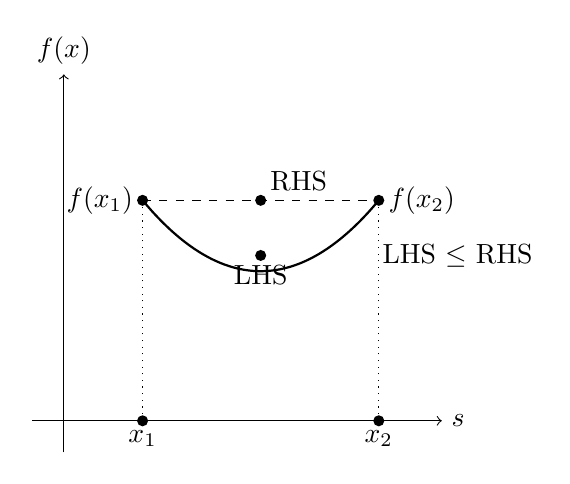
\begin{tikzpicture}[scale=2]
    % Axes
    \draw[->] (-0.2,0) -- (2.4,0) node[right] {$s$};
    \draw[->] (0,-0.2) -- (0,2.2) node[above] {$f(x)$};
  
    % Points on the x-axis
    \coordinate (X1) at (0.5,0);
    \coordinate (X2) at (2,0);
    \fill (X1) circle (1pt) node[below] {$x_1$};
    \fill (X2) circle (1pt) node[below] {$x_2$};
  
    % Function curve (convex parabola)
    \draw[domain=0.5:2,smooth,variable=\x,thick] plot ({\x},{0.8*(\x - 0.5)*(\x - 2) + 1.4});
  
    % Points on the function
    \coordinate (FX1) at (0.5,1.4);
    \coordinate (FX2) at (2,1.4);
    \fill (FX1) circle (1pt) node[left] {$f(x_1)$};
    \fill (FX2) circle (1pt) node[right] {$f(x_2)$};
  
    % RHS (linear interpolation)
    \draw[dashed] (FX1) -- (FX2);
  
    % Point on RHS (midpoint of the segment)
    \coordinate (RHS) at (1.25,1.4);
    \fill (RHS) circle (1pt);
    \node[above right] at (RHS) {RHS};
  
    % LHS point (on the function)
    \coordinate (LHS) at (1.25,1.05);
    \fill (LHS) circle (1pt);
    \node[below] at (LHS) {LHS};
  
    % Dashed lines from x1 and x2 to function
    \draw[dotted] (X1) -- (FX1);
    \draw[dotted] (X2) -- (FX2);
  
    % Inequality annotation
    \node at (2.5,1.05) {LHS $\leq$ RHS};
  \end{tikzpicture}
\end{center}
We can then expand the definition of convexity as follows:
\begin{definition}
    $f$ is strongly convex over $S$ if for any $x_1, x_2 \in S$ and $t \in [0,1]$, $f(tx_1 + (1-t)x_2) < tf(x_1) + (1-t)f(x_2)$
\end{definition}
A natural expansion of this is when $f$ is convex, then $f \left( \sum_{i = 1}^{n} t_i x_i \right) \leq \sum_{i = 1}^{n} t_i f(x_i)$ where $\sum_{i = 1}^{n} t_i = 1$ such that $t_i \geq 0$. We can also consider the following definition of convexity:
\begin{definition}
  Locally Convex: $f: \Omega \to \R$, where $f$ is convex over some $S \subseteq \Omega$
\end{definition}
\subsection{Taylor's Theorem}
We begin with an introduction of smoothness.
\begin{definition}
  A function is said to be $C^n$ if it is contionus and differentiable $n$ number of times. 
\end{definition}
Also a refresher on what the Taylor's Theorem in 1D is. 
\begin{definition}
  if $f: \R \to \R$ is $(k+1)$ times differentiable at $x = a$, then 
  \[
  f(x) = f(a) + \frac{\partial f(a)}{\partial x}(x-a) + \dots + \frac{1}{k!} \frac{\partial^k f(x)}{\partial x^k}(x-a)^k + \frac{L}{(k+1)!}(x-a)^{k+1}
  \]
  where 
  \[
  L = \sup_{\xi \in [x,a]} \left| \frac{\partial^{k+1} f(x)}{\partial x^k} \right|
  \]
\end{definition}
note that if $|x-a|$ is sufficiently small, we can discard the remainder the term (the one with the $L$ in it). Note that also that if the $(k+1)$ derivative is bounded, then we can approximate $f$ with the kth order polynomial. We can also consider the case of the special case of the third order taylor polynomial expansion. 
\begin{definition}
  For $f: \R^n \to \R$, and $f$ has a bounded 3rd deriative, the expansion is as follows
  \[
  f(x) = f(a) + \frac{\partial f(a)}{\partial x} (x-a) + \frac{1}{2}(x-a^T) H(a)(x-a) + \mathcal{O}(\|x-a\|^3)
  \]
  where we define
  \[
  H(a)_{ij} = \frac{\partial f(a)}{\partial x_i \partial x_j}
  \]
  where $H(a)$ is $n \times n$
\end{definition}
To illustrate the nature of the Hessian Matrix, we can visualize $f$ locally to see that we can use a contour map. The Hessian usually shows the directions of the biggest changes in direction, given by the Eigenvalues. \todo{Need to fix}


However, we can see that if our function is convex and smooth, then \emph{optimality is guarantted based on the local deriative}. We can see this in the following proof:
\begin{proof}
  if $f$ is convex and differentiable, we can see that if we let $a,b$ be in the domain of $f$. we can see that we are left with the following inequality. 
  \[
  f(b) \geq f(a) + \frac{\partial f(a)}{\partial x}(b-a)
  \]
  by the definition of convexity. If we choose $a$ such that $f'(a) = 0$, we see that we have guarnteed an optimal solution. 
\end{proof}
However, we can see that if we are working with a strongly convex differentiable solution, we can use the same assumptions as above to see in the following proof. 
\begin{proof}
  We are given that $f$ is strongly convex and differentiable. Thus, we can see that for the following taylor expansions 
  \[
  f(b) \geq f(a) + \frac{\partial f(a)}{\partial x}(b-a) + \frac{a}{2} \|b - a\|_2^2
  \]
  We see that we can choose a point such that $\frac{\partial f(a)}{\partial x} = 0$, which implies that 
  \begin{align*}
    f(b) &\geq f(a) + \frac{a}{2} \|b - a\|^2\\
    \implies  & f(b)  > f(a), \forall b, b \neq a
  \end{align*}
  Since we know that the function is strongly convex and thus, we know that for any point $b$ and $a$. the last inequality holds, we can see that we have indeed foound the unique optimizer.
\end{proof}
\begin{remark}
  Strongly convex implies strictly convex, but not the other way around. 
\end{remark}
\subsection{Applications of convexity}
Consider the following:
\[
f(x) = \frac{1}{2} ax^2 - bx, a > 0
\]
and consider the following:
\begin{align*}
  f(x) &= \frac{1}{2}ax^2 - bx\\
  f(y) - f(x) &= \frac{1}{2}a(y^2 - x^2) - b(y-x)
\end{align*}
\section{Lecture 10: Introduction to Gradient Descent}
As noted before, we can see that when we are given a convex function, say $f(x) = 0.5ax^2 - bx$ where $a > 0, b > 0$, we are left with a convex function where we can use the deriative of the function to solve for the extrema values. Now we aim to expand this out to a multivariate case. The anaolgue of a positive value matrix is a \emph{positive definite matrix}, or where all the eigenvalues are all positive. We can show that if $M$ is a positive definite symmetric matrix, than $f$ is a strongly convex function. 
\begin{proof}
  We are given the function $f(x) = \frac{1}{2} M - b^T x$, which is a natural analogue to the 1-d case. We can see that $M = U \Lambda U^T$ , where $U$ is orthogonal. Thus, we can see that
  \[
  f(x) = \frac{1}{2}x^T U \Lambda U^T x - b^T(UU^T)x
  \]
  and let $\tilde{x} = U^Tx$ and $\tilde{b} = U^Tb$. Thus, we are left with the following:
  \[
  \sum_{i=1}^n \frac{1}{2} \lambda_{ii} \tilde{x}_i^2 - \tilde{b}_i \tilde{x}_i
  \]
  which is equiavlent to the 1d case, where 
  \[
  \sum_{i = 1}^{n} f_i(\tilde{x}_i)
  \]
  where each $f_i$ is strongly convex. Since the sum of strongly convex functions are still strongly convex, then we know that $f$ is strongly convex. 
\end{proof}
\begin{remark}
  We are familar with the least squares problem, or when 
  \[
  x = \arg \min_{x} \|Ax -b \|^2
  \]
  \todo{Fill in this in later after confirming }
\end{remark}
\subsection{How to solve for the extrema}
If we are given a strongly convex function where there exists a $x$ such that $\nabla f(x) = 0$. then x must be the unique minimizer. On a computer, we have the following methods:
\begin{itemize}
  \item \textbf{Netwon's Type Method}: Note that we are interested in solving the system of equations where \[
  \nabla f(x) = Mx - b
  \]
  where $M$ denotes the Jacobian of a matrix. To compute this problem, we see that we have to solve for $x^* = M^{-1}b$, which is compuationally expensive, as proved before it takes $\mathcal{O}(n^3)$ to solve such a system. 
  \item \textbf{Gradient based minimization thorugh iterative algorithm}: We use the gradient multiplized by some arbitary value to travel down the fucntion to see if we can converge on the minima value. For example, we want a solution that converges to the optimal value, say $x^*$. 
\end{itemize}
Ultimately for the gradient method, we want to create a sequence of $x$ that converegs to the optimal value $x^*$. To do so, we must define some sort of relationship between successive values in the sequence. Therefore, we must introduce an \emph{updating scheme}. We define the updating scheme as follows:
\[
x^{k+1} = x^k - s_k Df(x^k)
\]
where $s_k$ is the step size. Now a natural question that may follow is "How do we choose the step size?". 


This depends heavily on the shape and structure of the function. Consider the strongly convex framework that we are very familar with. We can define an objective function, where we want to minimize the difference in function values of the sequence values and the actual minimizer. Consider the following:
\[
f(x) = \frac{1}{2}(x-x^k)^T < (x - x^k) + \xi 
\]
where $\xi$ is some constant. We can see that the above simplifes to:
\[
f(x) = \frac{1}{2}\|x - x^k\|^2_M + \xi
\]
without a loss of generality, we can set the above function as $f(x) = \frac{1}{2}\|x-x^k\|^2_M$. If we want to show that the fucntion linear converges to some magnitude, we can see that:
\[
\|x^{k+1} - x^*\| \leq C \|x^k - x^*\|^q
\]
We have two cases, linear convergence and quadratic convergence. Linear convergence is when $q = 1$ and $C \in [0,1]$. Similarly, quadratic convergence is when $q = 2$ and $C > 0$. We begin to prove that this gradient descent has linear convergence is we pick a step size such that $s_k \in (0, \frac{1}{\lambda_{max}(M)})$ 
\begin{proof}
  For notational sake, let $M$ be the Jacobian matrix and. Note that:
  \[
  \nabla f(x) = Mx - b
  \]
  Thus, 
  \begin{align*}
    \|x^{k+1} - x^*\|^2 &= \|x^k - s(Mx^k - b) - x^*\|^2\\
    &= \|x^k - x^* -s(Mx^k - Mx^*)\|^2\\
    &= \|(I - sM)(x^k - x^*)\|^2
  \end{align*}
\end{proof}
\end{document} 